% 建议使用 XeLaTeX 或 LuaLaTeX 编译(中文与公式支持更佳)
\documentclass[UTF8,zihao=-4]{ctexart}

\usepackage[a4paper,margin=2.5cm]{geometry}
\usepackage{amsmath, amssymb, amsthm}
\usepackage{bm}
\usepackage{hyperref}
\usepackage{graphicx}
\usepackage{caption}
\usepackage{listings}
\usepackage{xcolor}
\usepackage{float}
\usepackage{placeins}
\graphicspath{{figures/}}

\lstdefinestyle{code}{
  basicstyle=\ttfamily\small,
  numbers=left,
  numberstyle=\tiny,
  numbersep=8pt,
  keywordstyle=\color{blue},
  commentstyle=\color{teal!70!black},
  stringstyle=\color{orange!70!black},
  showstringspaces=false,
  breaklines=true,
  frame=single,
  framerule=0.3pt,
  rulecolor=\color{black!15}
}
\lstset{style=code}

\title{REINFORCE 策略梯度:原理、公式、应用与实战}
\author{}
\date{\today}

\begin{document}
\maketitle

\section{引言}
REINFORCE(蒙特卡洛策略梯度)通过完整轨迹的回报来更新策略参数,其梯度估计无偏、实现简单,是策略梯度方法的基础。算法以 \(\sum_t \nabla_\theta \log \pi_\theta(a_t\mid s_t) G_t\) 形式累积梯度,因此方差较大但便于理论分析与扩展。

\section{原理与公式}
\subsection{蒙特卡洛策略梯度}
从策略 \(\pi_\theta\) 采样轨迹 \(\tau\) 后,REINFORCE 梯度估计为:
\begin{equation}
\nabla_\theta J(\theta) = \mathbb{E}_{\tau \sim \pi_\theta}\Big[ \sum_{t=0}^{T-1} \nabla_\theta \log \pi_\theta(a_t\mid s_t)\, G_t \Big],
\end{equation}
其中回报 \(G_t = \sum_{k=t}^{T-1} \gamma^{k-t} r_{k+1}\)。

\subsection{基线与方差削减}
引入基线 \(b(s_t)\) 不改变期望梯度:
\begin{equation}
\nabla_\theta J(\theta) = \mathbb{E}\Big[ \sum_t \nabla_\theta \log \pi_\theta(a_t\mid s_t)\, (G_t - b(s_t)) \Big].
\end{equation}
常见基线包括常数、值函数估计或滚动平均,有助于降低梯度方差。

\subsection{算法步骤}
\begin{enumerate}
  \item 使用当前策略采样若干条轨迹;
  \item 计算每个时间步的回报 \(G_t\)(可使用 reward-to-go 减少方差);
  \item 更新参数:\(\theta \leftarrow \theta + \alpha \sum_t \nabla_\theta \log \pi_\theta(a_t\mid s_t)(G_t - b(s_t))\);
  \item 可选:同步更新基线或价值估计。
\end{enumerate}
由于依赖完整回报,REINFORCE 方差较高但实现简单,是许多改进方法的起点。

\section{应用与技巧}
\begin{itemize}
  \item \textbf{回合式任务}:回合长度适中、奖励稀疏的环境。
  \item \textbf{课程学习}:先用 REINFORCE 预热,再切换到 Actor-Critic。
  \item \textbf{离散策略}:处理多臂老虎机、离散动作控制。
  \item \textbf{实用建议}:对回报做归一化,引入基线,调整学习率,并使用 reward-to-go 或优势函数降低方差。
\end{itemize}

\section{Python 实战}
脚本 \texttt{gen\_reinforce\_figures.py} 在网格世界上运行 REINFORCE,并采用滑动平均基线,输出回报曲线与状态访问频率热力图。
\begin{lstlisting}[language=Python,caption={脚本 gen_reinforce_figures.py 片段}]
returns = compute_returns(rewards, gamma)
for (state, action), G_t in zip(trajectory, returns):
    probs = softmax(theta[state])
    grad = -probs
    grad[action] += 1.0
    baseline[state] += baseline_lr * (G_t - baseline[state])
    theta[state] += alpha * grad * (G_t - baseline[state])
\end{lstlisting}

\section{实验结果}
\begin{figure}[H]
  \centering
  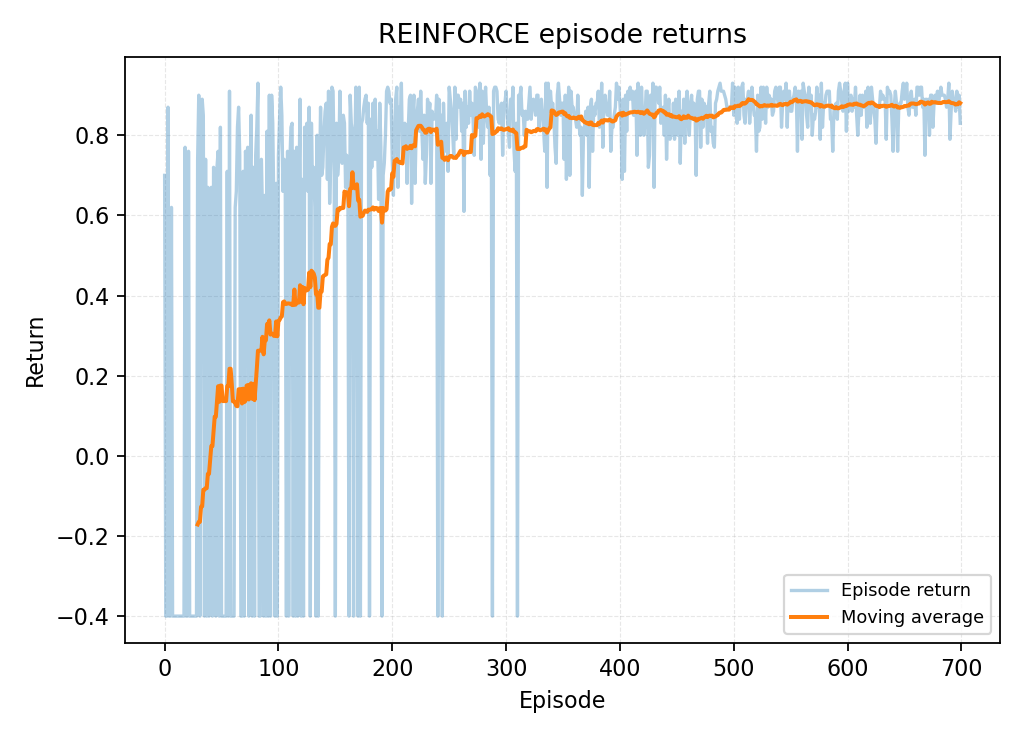
\includegraphics[width=0.8\linewidth]{reinforce_returns.png}
  \caption{REINFORCE 回报曲线与滑动平均}
  \label{fig:reinforce_returns_cn}
\end{figure}

\begin{figure}[H]
  \centering
  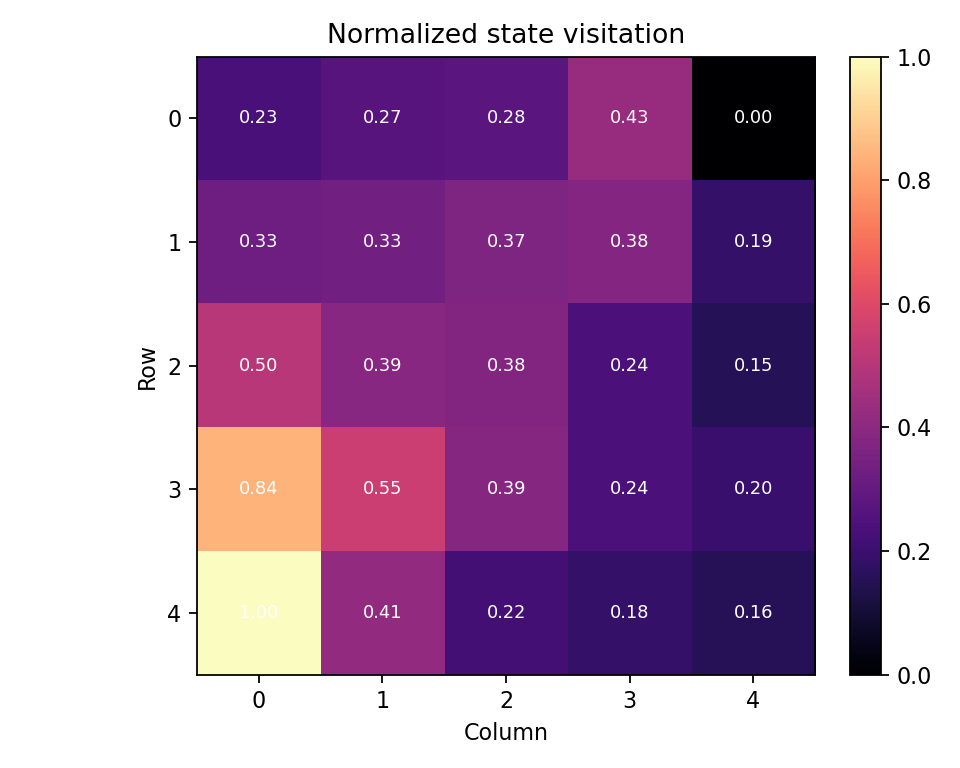
\includegraphics[width=0.82\linewidth]{reinforce_state_visitation.png}
  \caption{训练后状态访问热力图,显示策略倾向的路径}
  \label{fig:reinforce_state_visitation_cn}
\end{figure}

\FloatBarrier
\section{总结}
REINFORCE 提供简单无偏的策略梯度估计,但需依赖方差削减与学习率调节。通过基线、归一化与批量采样,可显著提升训练稳定性。示例展示了回报随训练改善以及策略如何集中于高回报路径。

\end{document}